\documentclass{beamer} %for at du kan lave en prÊsintation skal du skriove beamer i class% 
\usetheme{Marburg} %her bestemmer du designet fx madrig du kan ogs bestemme om der skal vises under katagorier%
\setcounter{tocdepth}{1}

\usepackage[latin1]{inputenc} %standart%
\usepackage[english]{babel}%standrat%
\usepackage{amsmath,amsfonts,amssymb}%standrat%
\usepackage[]{subfig}
\usepackage{sadlist}
\usepackage{tabularx}
\usepackage[]{graphicx}

\author{s305a}
\institute{Aalborg University}
\title{Hopla Helpdesk}
\subtitle{Programming}

\begin{document}

\section*{Frontpage}
\begin{frame}
\titlepage
\end{frame}
\subsection*{Disposition}
\begin{frame}{Disposition}
\begin{itemize}
	
	
	\item Introduction
	\begin{itemize}
		\item Purpose 
		\item Application Definition 
	\end{itemize}
	\item<2-> OOAD 
	\begin{itemize}
		\item<2->  Roles 
		\item<2->  Use Cases 
		\item<2->  Interfaces 
		\item<2->  Quality Goals 
		\item<2->  Component Architecture 
		\item<2->  Model Component	
	\end{itemize}
	\item<3-> Implementation 
	\begin{itemize}
		\item<3-> Development Method 
		\item<3-> Submit Problem 
		\item<3-> Solve Problem 
		\item<3-> Statistics 
	\end{itemize}	
	\item<4-> Testing 
	\begin{itemize}
		\item<4-> Test Methods 
	\end{itemize}
	\item<5-> Conclusion 
\end{itemize}
\end{frame}
\section{Purpose}
\begin{frame}{Purpose}

\begin{itemize}
	\item \textbf{Productivity:} Improve the problem solvers productivity
	\begin{itemize}
		\item Communication
		\item Environment
		\begin{itemize}
			\item Institutions
			\item Departments
			\item Different areas of responsebility
			\end{itemize}
	\end{itemize}
\end{itemize}


\end{frame}

\section*{Application Definition}
\begin{frame}{Application Definition}
\begin{itemize}
\item The application must be web-based so that we can create an application capable of running without prior installation.
\item The application contains prioritized tags, enabling us to determine the importance of problems
\item The application keeps track of the estimated completion time of the problem along with comments and which employee is responsible for solving the problem.
This enables us to create statistics about problem solving efficiency and individual employees.
\end{itemize}
\end{frame}

\begin{frame}{Application Definition}
\begin{itemize}
\item The application is able to save and suggest prior problems and their solutions to users.
\item The application takes into account, the workload of the employees to estimate how long a problem will take to solve.
\item The application contains nothing but dynamic data within the problem domain, so that the application can run in different environments.
\item The application contains a structure that can handle problems, departments, categories, tags, regular personnel, supervisors and staff members.
\end{itemize}
\end{frame}

\section{OOAD}
\begin{frame}
\begin{center}
\huge
Object Oriented Analysis \& Design
\end{center}
\end{frame}
	\subsection{Roles}
\begin{frame}{Roles}

\begin{itemize}
\item Client
	\begin{itemize}
	\item Regular end-user
	\end{itemize}
\item Staff
\item Admin
\end{itemize}

\end{frame}
	\subsection{Use Cases}
\begin{frame}{Use Cases}

\begin{figure}[htbp]
	\begin{center}
	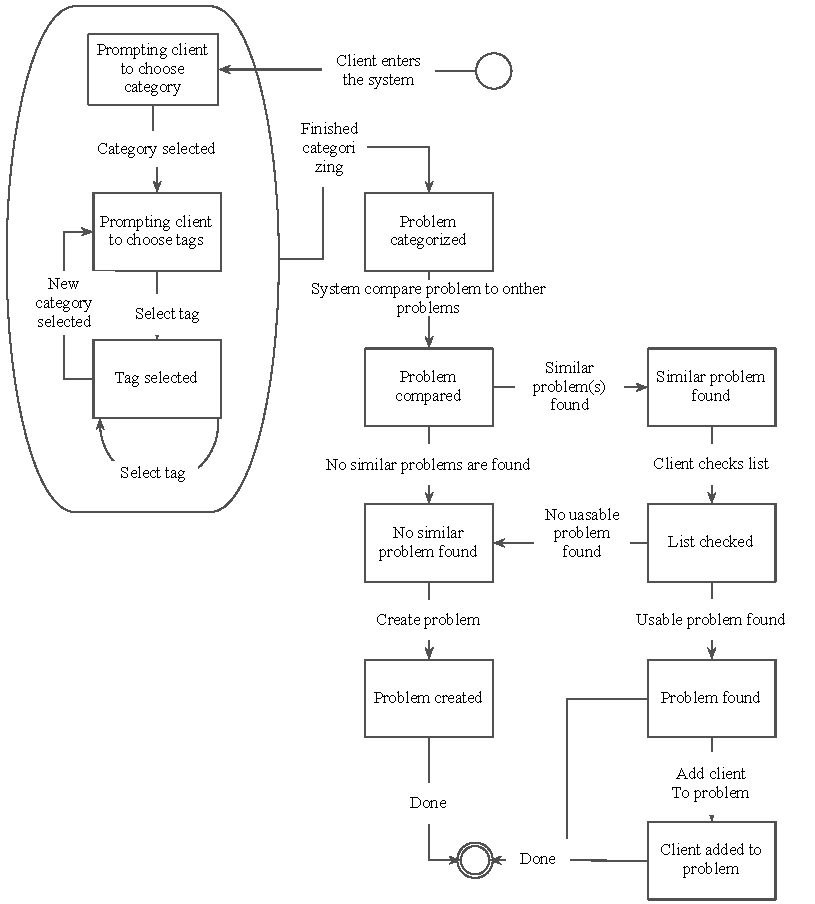
\includegraphics[height=200pt]{input/sad/submit_problem_use_case.pdf}
	%\caption{default}
	%\label{default}
	\end{center}
\end{figure}

\end{frame}
	\subsection{Interfaces}
\begin{frame}

\end{frame}
	\subsection*{Quality Goals}
\begin{frame}
\tiny
\begin{sable}{0.2}{0.5}{Definition of criteria}{fig:defOfCrit}
 \shfone{Criterion}&\shftwo{Definition} \\
\hline \\
  %Usable&The end user can easily use the application \\ \\
  %Secure&Precautions against unauthorized access \\ \\
  %Efficient&How well the resources available are being used \\ \\
  Consistence&How correct the data in the model is \\ \\
  %Reliable&The degree of the applications accessibility \\ \\
  %Maintainable&The cost of locating and fixing application errors \\ \\
  Testable&The cost to ensure that the application performs intentionally \\ \\	
	Flexible&How easily the application can be setup to fit the structure of an institution. \\ \\  %Flexible&The cost for the end user to modify the system after deployment \\ \\
	%Comprehensible&How easy it is for the end user to understand the application \\ \\
	Comprehensible&How easy it is to understand the application \\ \\

  %Reusable&The potential for using parts of this application in another application \\ \\
  %Portable&How much effort needed to change the platform of the application \\ \\
  %Interoperable&How well the application cooperates with other applications \\
\end{sable}
\end{frame}


\begin{frame}
\tiny
\begin{figure}[]
		\begin{tabular}{| l | m{0.135\textwidth} | m{0.135\textwidth}|} \hline
 & Very  Important& Important \\ \hline

Consistence  				&& \multicolumn{1}{c|}{$\checkmark$} 		\\ \hline
Testable  					&& \multicolumn{1}{c|}{$\checkmark$} 		\\ \hline
Flexible  					& \multicolumn{1}{c|}{$\checkmark$} 		\\ \hline
Comprehensible  		&& \multicolumn{1}{c|}{$\checkmark$} 		\\ \hline
	
		\end{tabular}
	\label{fig:prioritizedCrit}
\end{figure}

\end{frame}
	\subsection{Component Architecture}
\begin{frame}{Component Architecture}


		\begin{figure}[p]%
		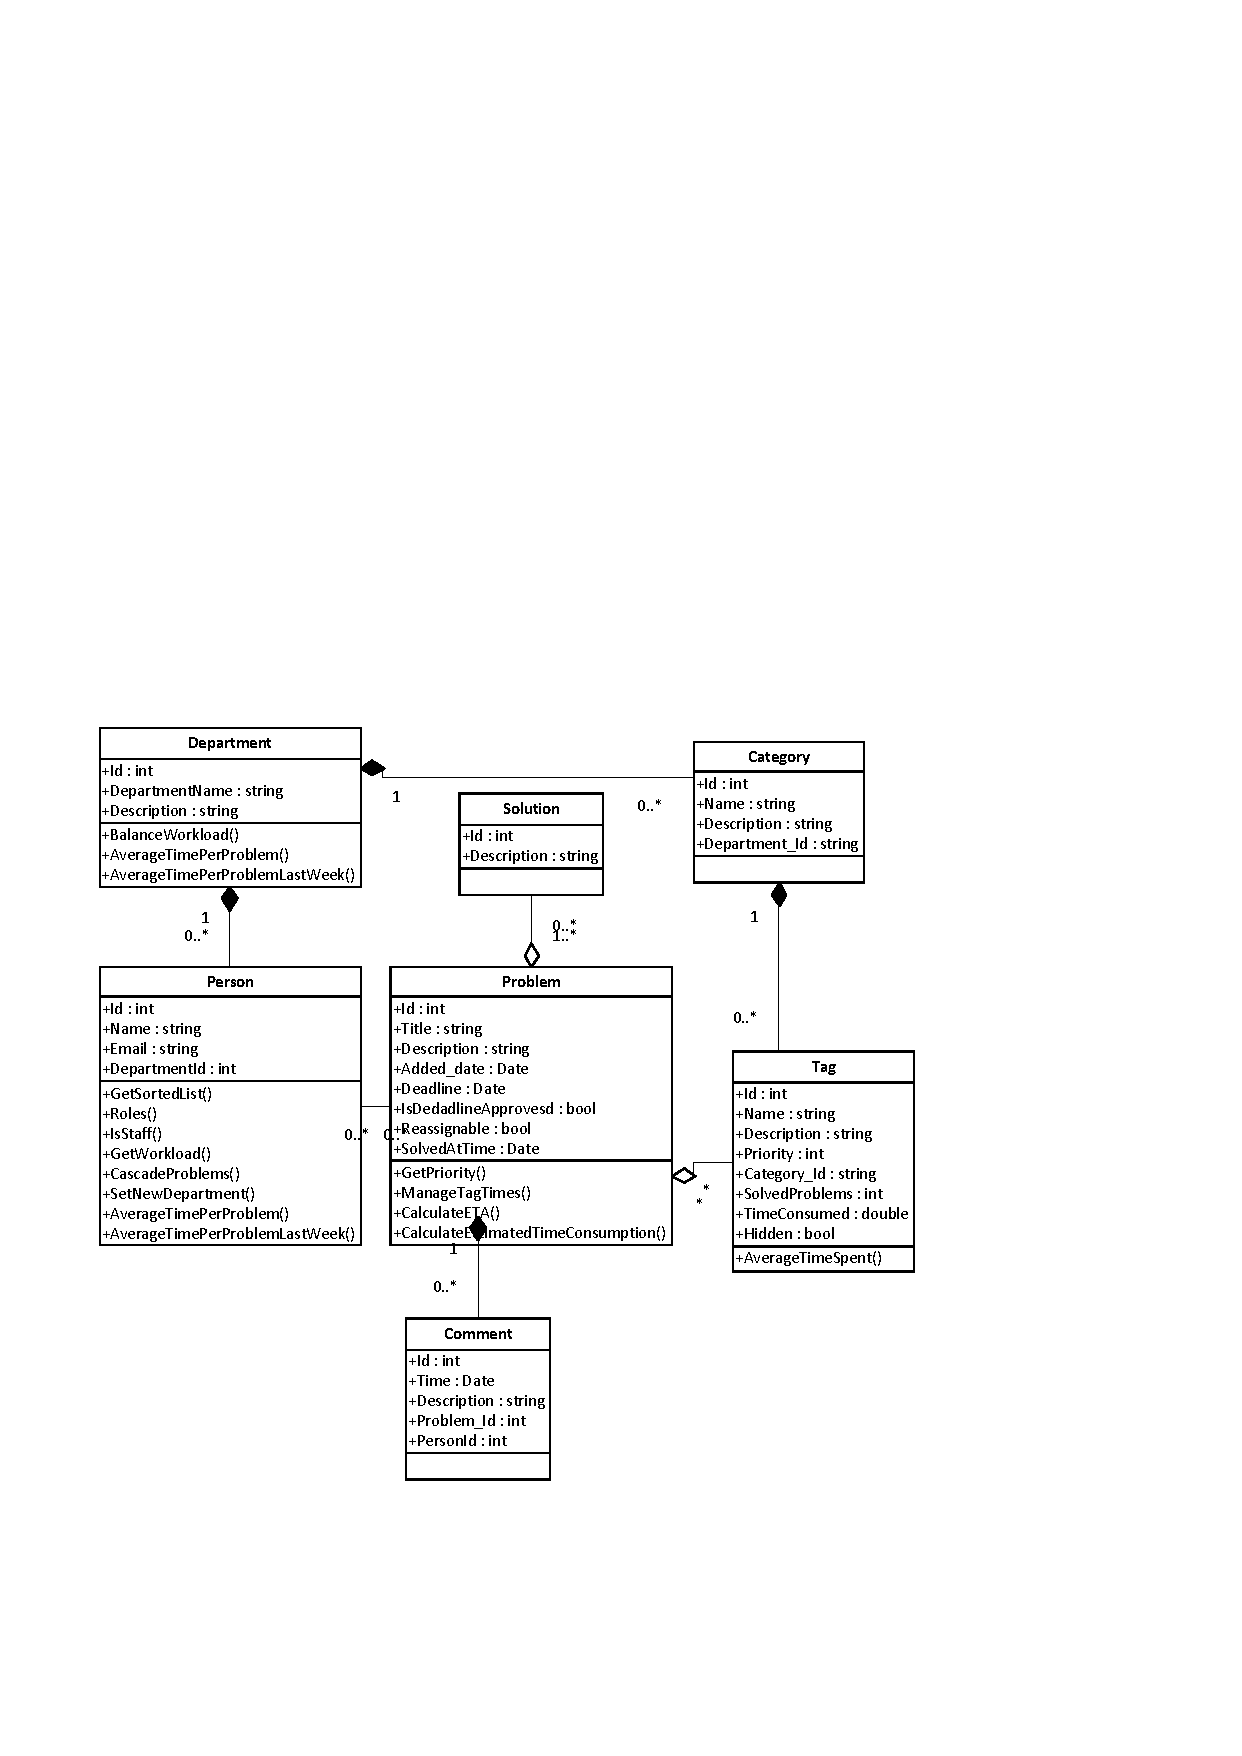
\includegraphics[clip=true, height=1.0\textwidth, trim=0.5cm 5cm 7.5cm 7cm]{input/ClassDiagramV2.pdf}%
		\end{figure}


\end{frame}

	\subsection{Model Component}
\begin{frame}{Model Component - Figure 8.1 p.46}
	
	\begin{figure}[p]%
	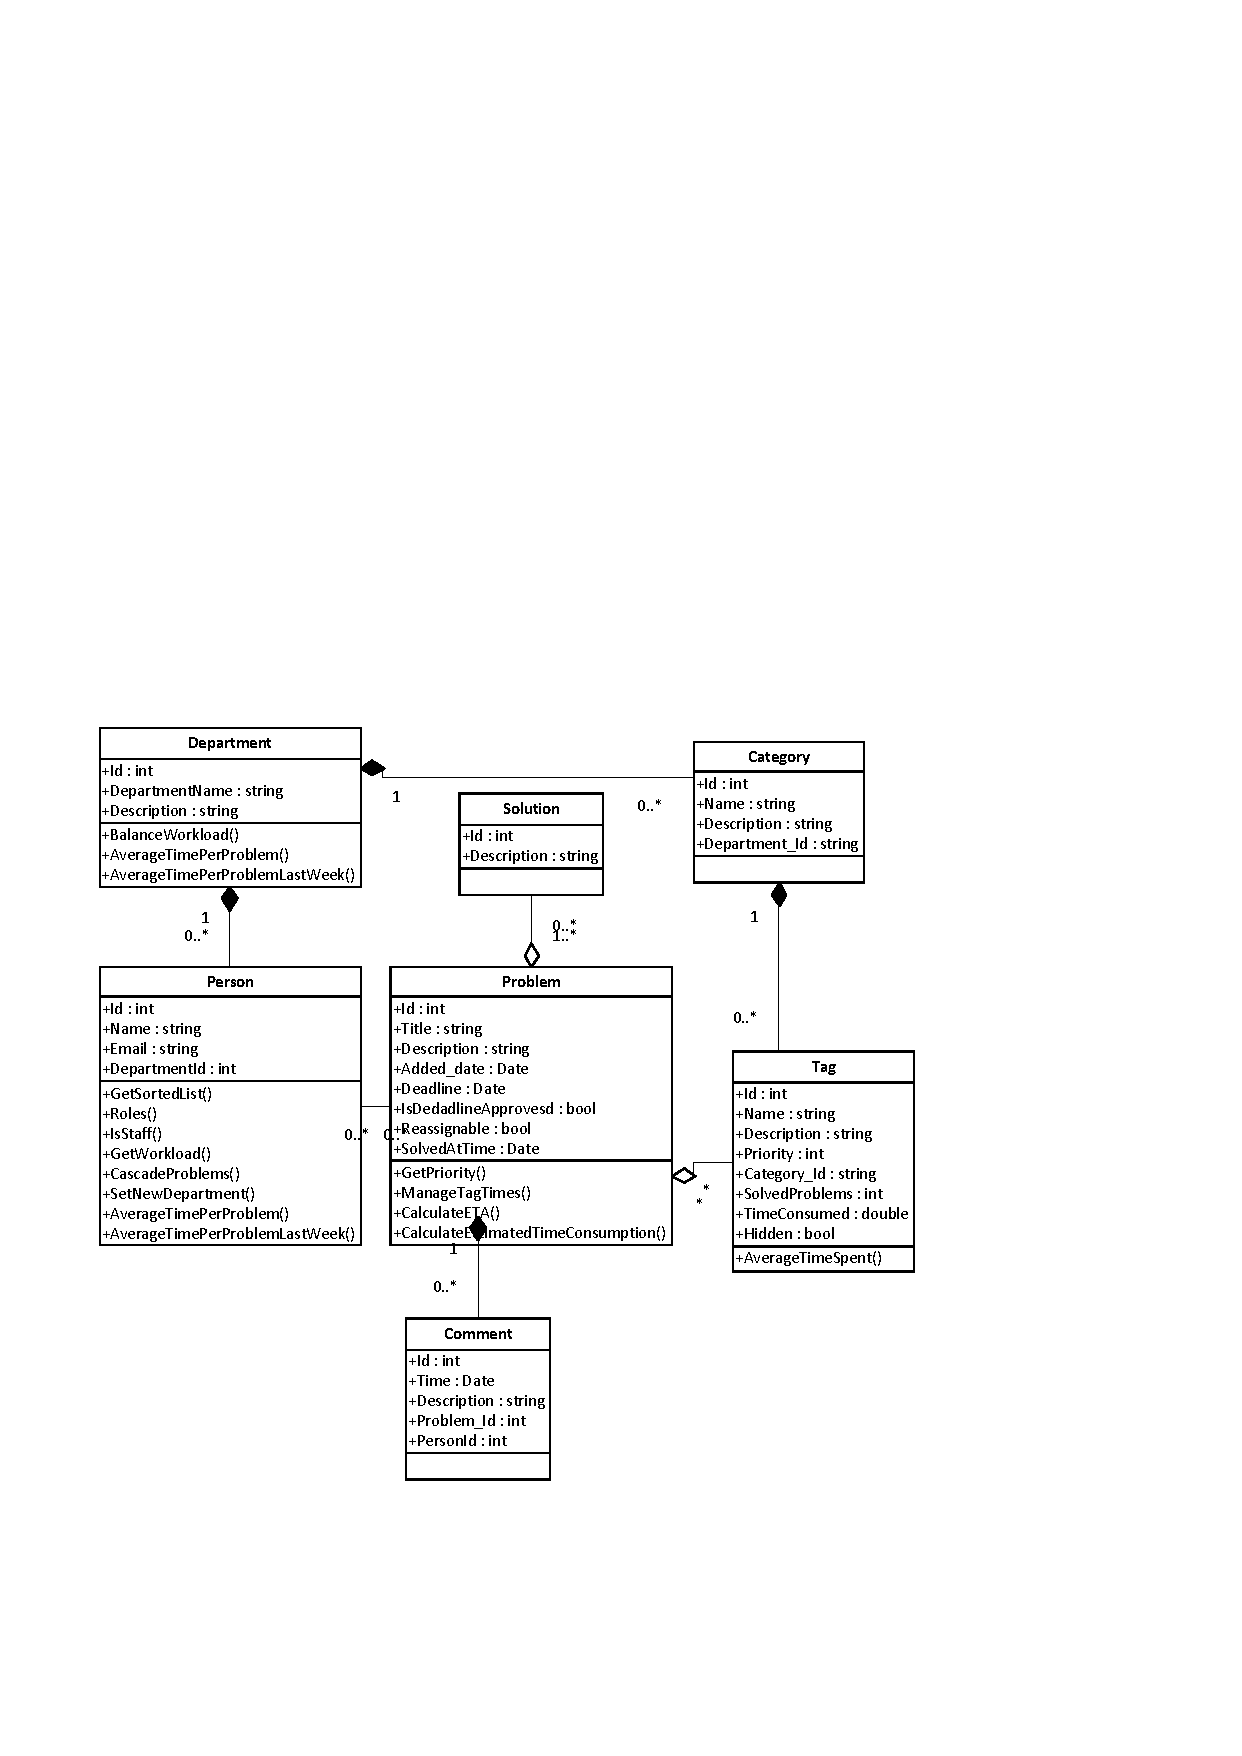
\includegraphics[clip=true, height=1.0\textwidth, trim=0.5cm 5cm 7.5cm 7cm]{input/ClassDiagramV2.pdf}%
	\end{figure}
	
\end{frame}

\section{Implementation}
\begin{frame}
\begin{center}
\huge
Implementation
\end{center}
\end{frame}
\subsection{Development Method}
\begin{frame}{Development Method}
\begin{itemize}
	\item Waterfall
	\item Scrum
	\item Extreme Programming
\end{itemize}
\end{frame}
\begin{frame}{Development Method}
\begin{itemize}
	\item Scrum
	\begin{enumerate}
		\item Daily planning
		\item Sprints
	\end{enumerate}
	\item Extreme Programming
	\begin{enumerate}
		\item Small releases
		\item Implement new features
		\item Collective ownership
		\item No Overtime
		\item Coding standards
	\end{enumerate}
\end{itemize}
\end{frame}
\begin{frame}
\begin{figure}[htbp]
\begin{center}
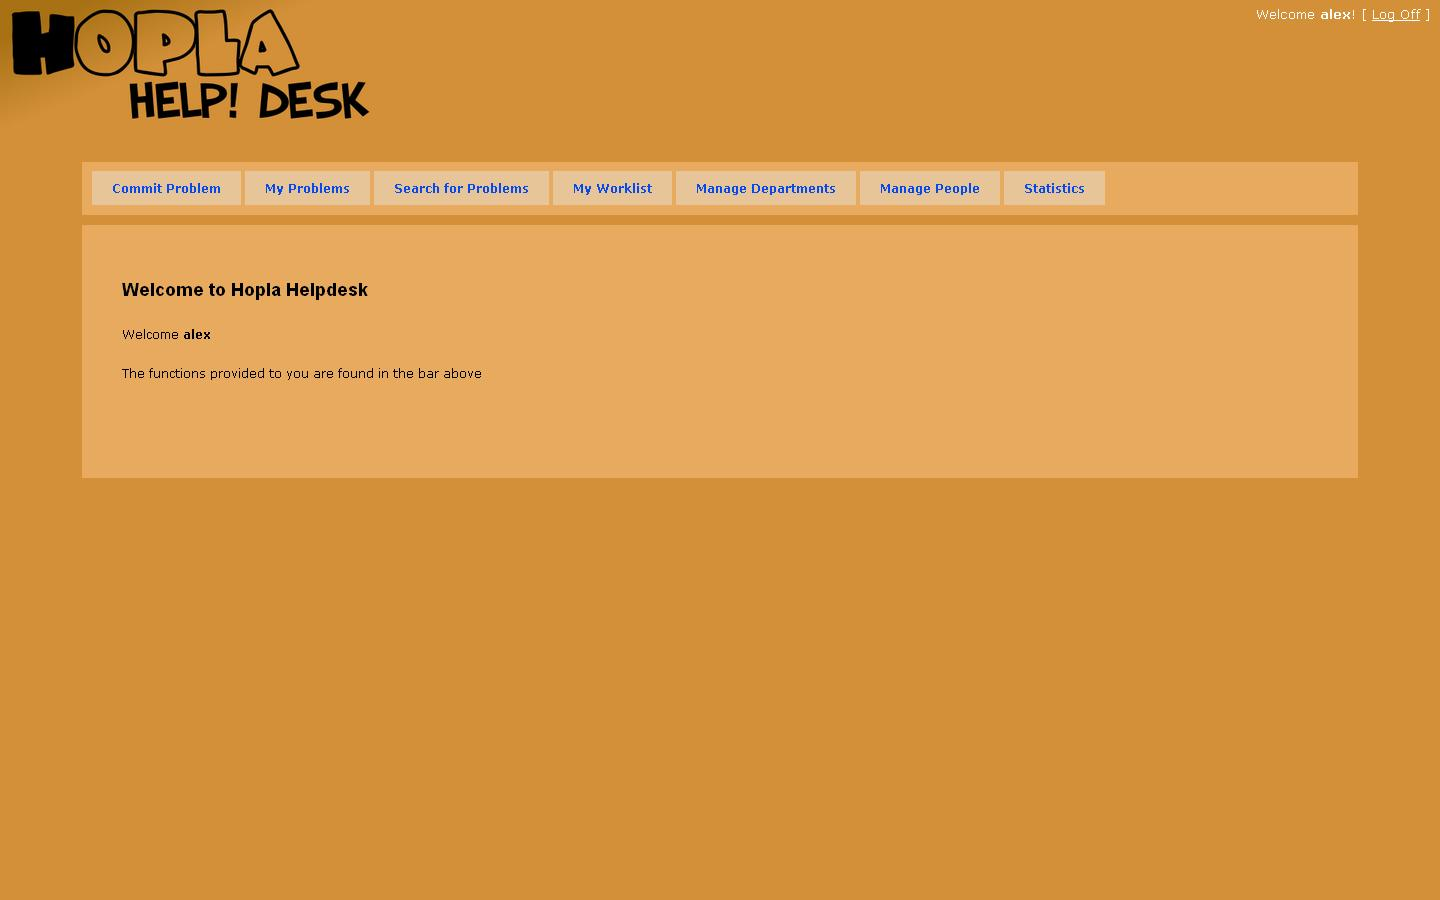
\includegraphics[]{input/search/home.JPG}
\caption{default}
\label{default}
\end{center}
\end{figure}

\end{frame}

\begin{frame}

\begin{figure}[htbp]
\begin{center}
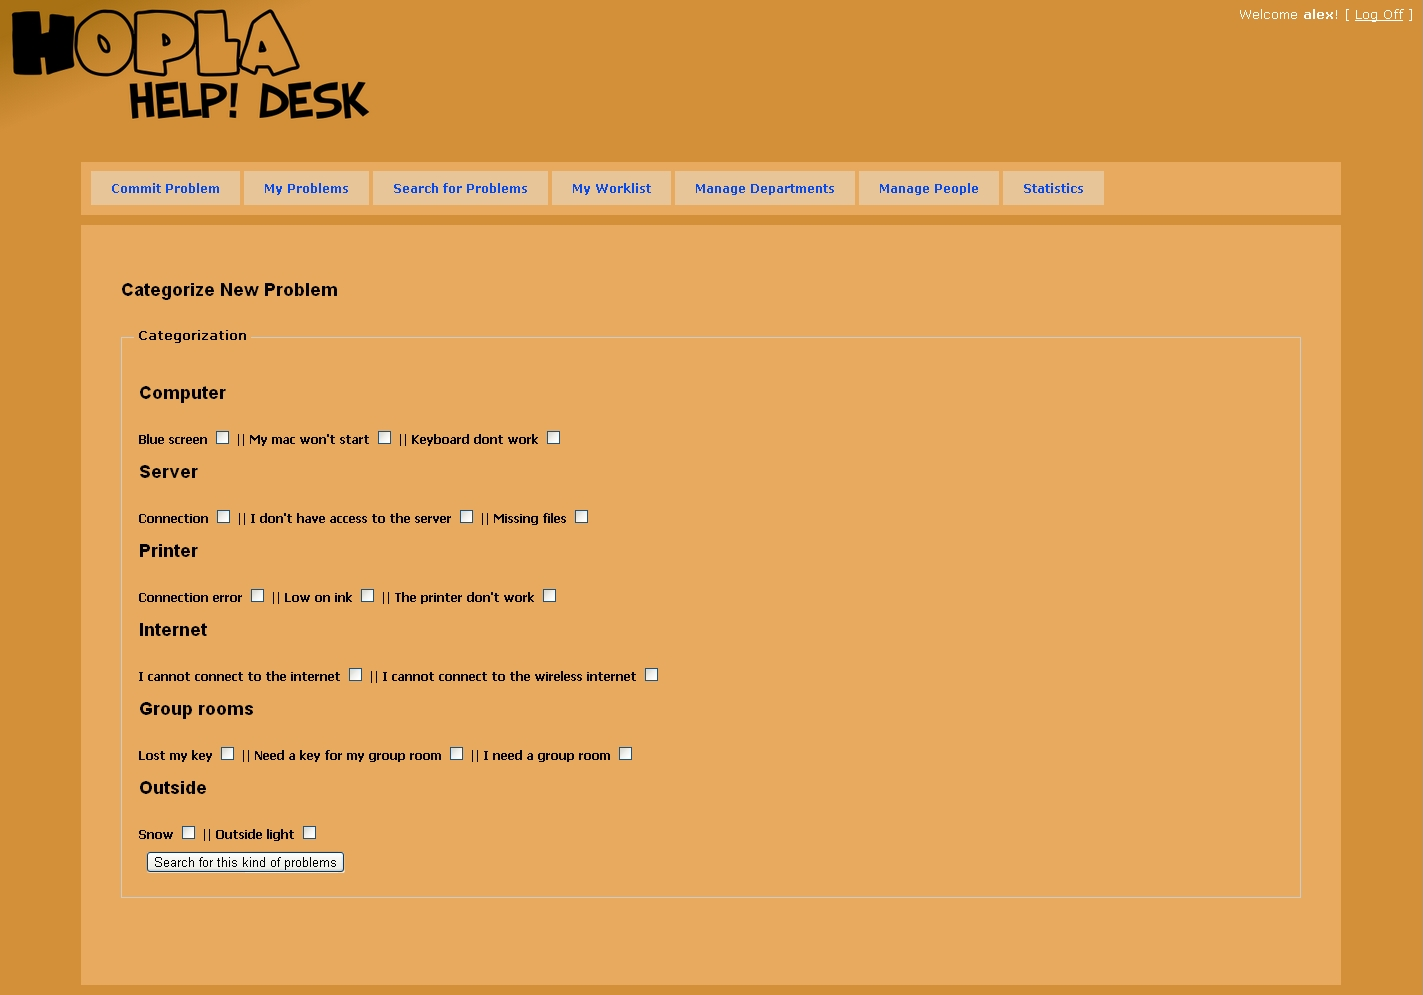
\includegraphics[]{input/search/commit.png}
\caption{default}
\label{default}
\end{center}
\end{figure}

\end{frame}

\begin{frame}

\begin{figure}[htbp]
\begin{center}
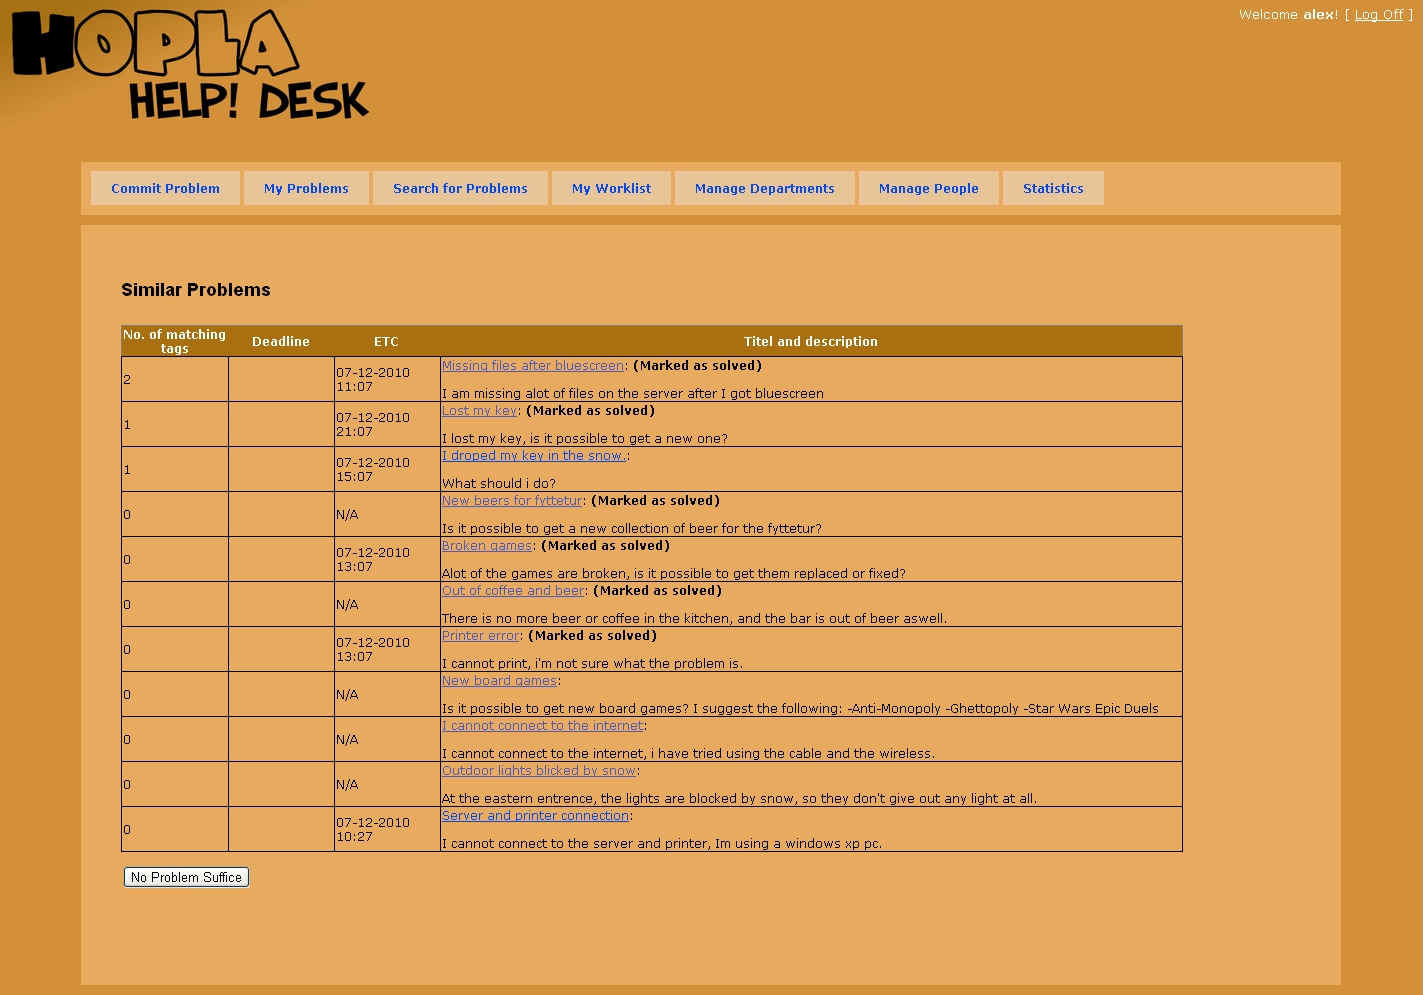
\includegraphics[]{input/search/similarProblems.png}
\caption{default}
\label{default}
\end{center}
\end{figure}

\end{frame}

\begin{frame}

\begin{figure}[htbp]
\begin{center}
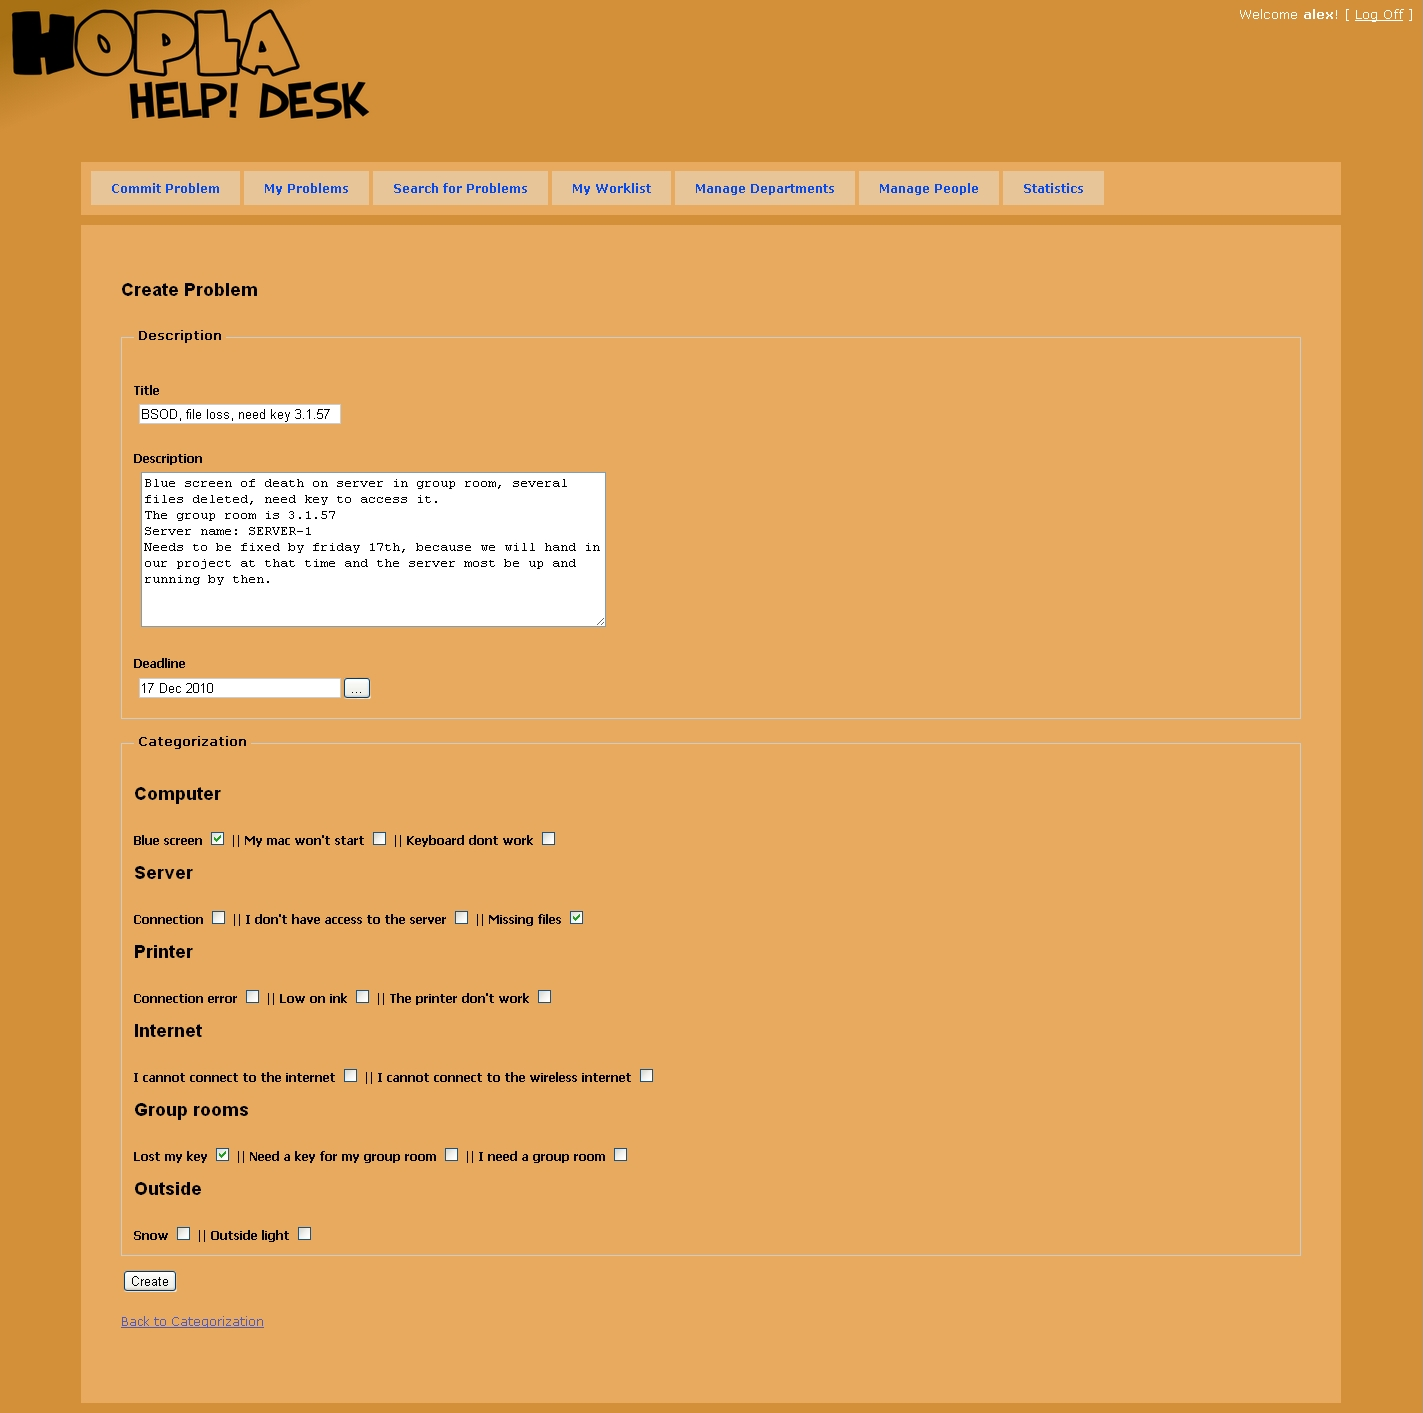
\includegraphics[]{input/search/newProblem.png}
\caption{default}
\label{default}
\end{center}
\end{figure}

\end{frame}
% The interresting here is the search, we try search a set of problems

\begin{frame}
\subsection{The Search}
\begin{itemize}
\item Tags to search: Computer + Bluescreen
\item Minimum number of problems to find: 3
\end{itemize}

\end{frame}



\begin{frame}
\subsection{The Search}
\begin{itemize}
\item Tags to search: Computer + Bluescreen
\item Minimum number of problems to find: 3
\end{itemize}

\end{frame}


\subsection{Solve Problem}
\begin{frame}{Solve Problem}
\begin{figure}[H]
	\centering
		\includegraphics[width=1.00\textwidth, clip=true, trim=4cm 10.5cm 8cm 8cm]{input/alex_before.png}
	\label{fig:alex_before}
\end{figure}

\begin{figure}[H]
	\centering
		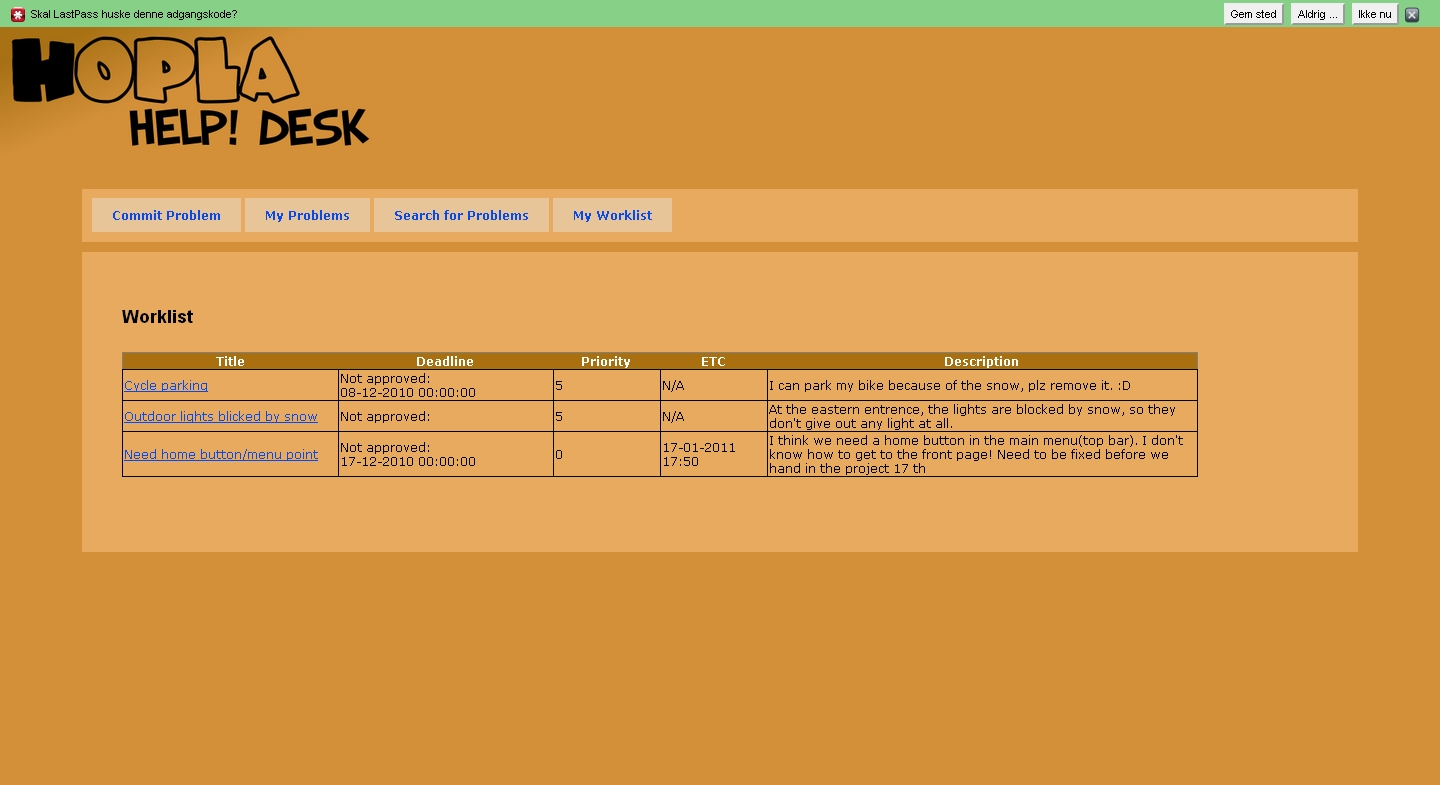
\includegraphics[width=1.00\textwidth, clip=true, trim=4cm 10.5cm 8cm 9cm]{input/magnus_before.png}
	\label{fig:magnus_before}
\end{figure}
\end{frame}

\begin{frame}{Solve Problem}
\begin{figure}[H]
	\centering
		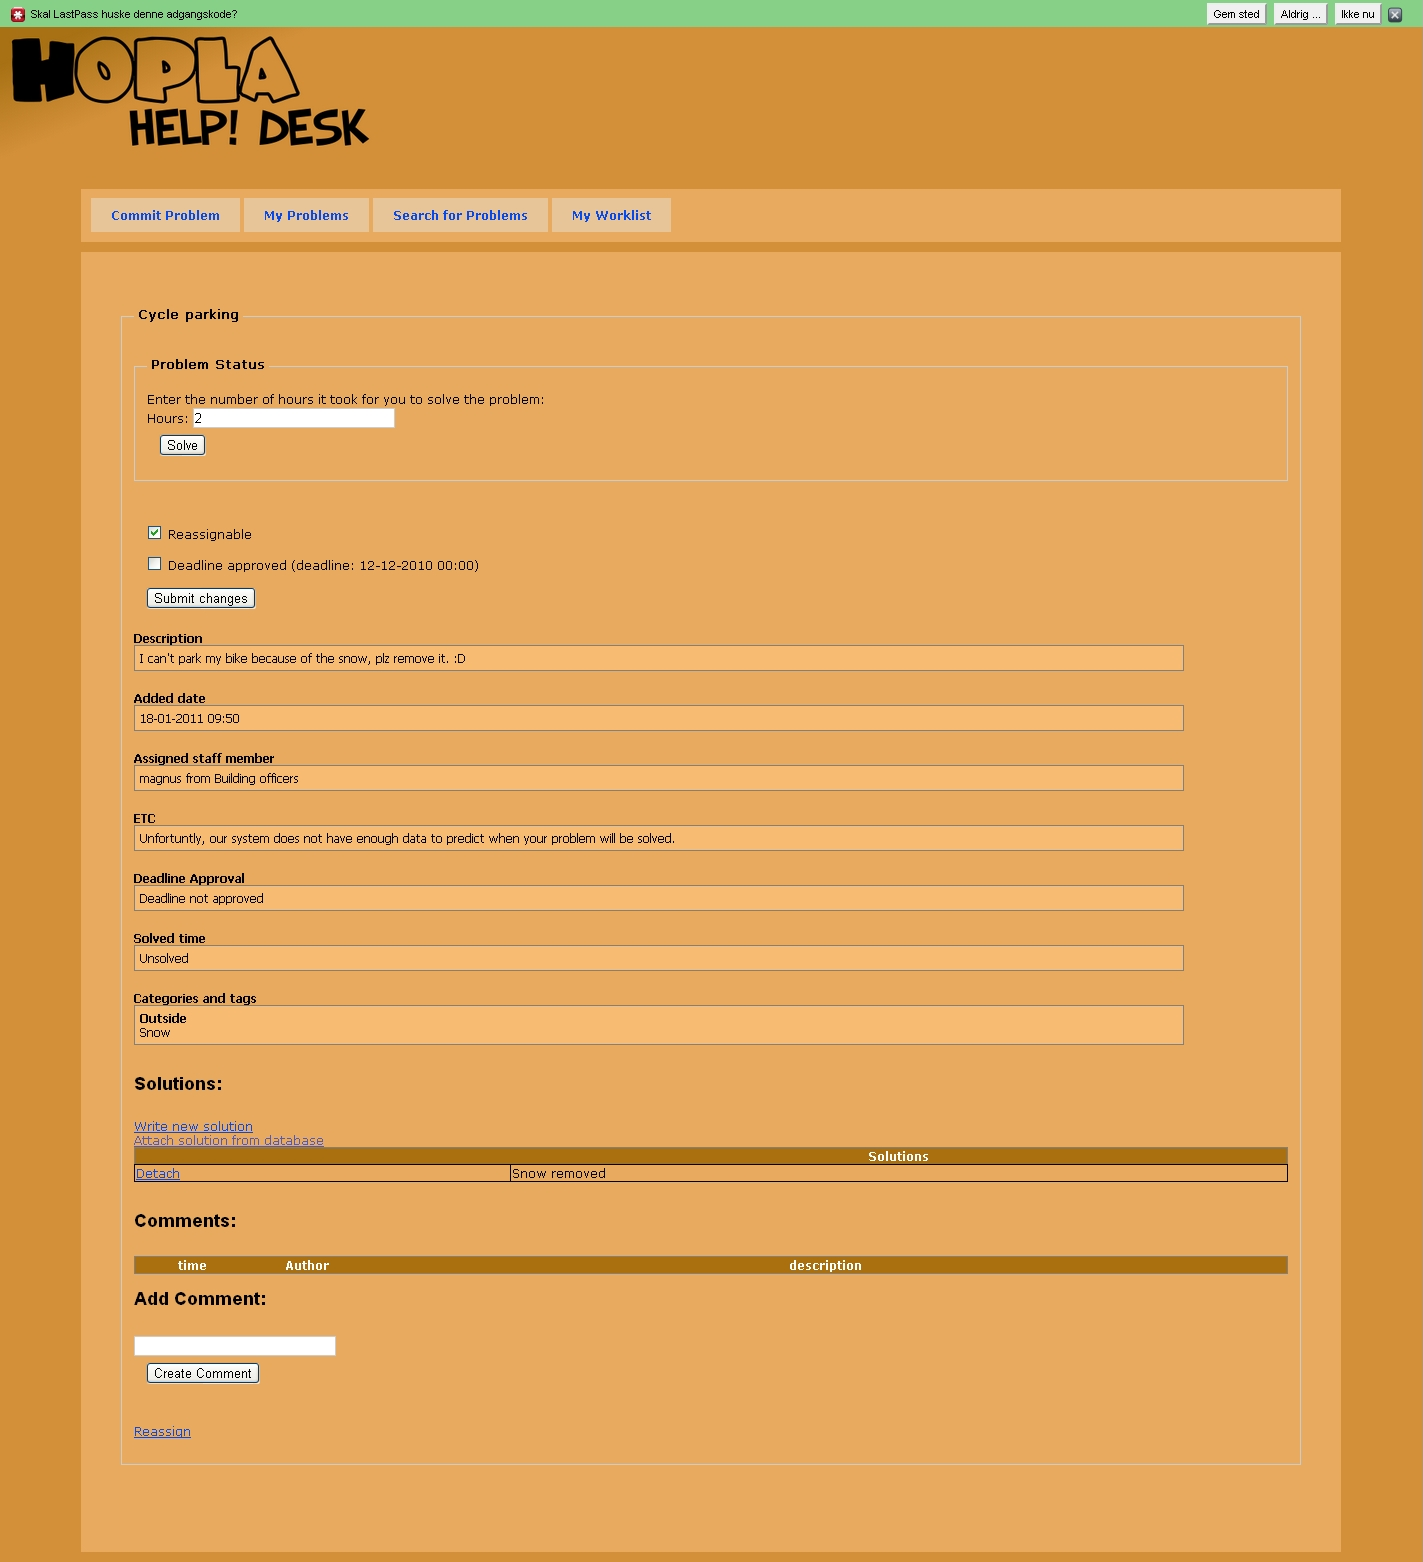
\includegraphics[width=0.90\textwidth, clip=true, trim=4cm 12.5cm 8cm 9.5cm]{input/magnus_solve.png}
	\label{fig:magnus_solve}
\end{figure}
\end{frame}

\begin{frame}{Solve Problem}
\begin{figure}[H]
	\centering
		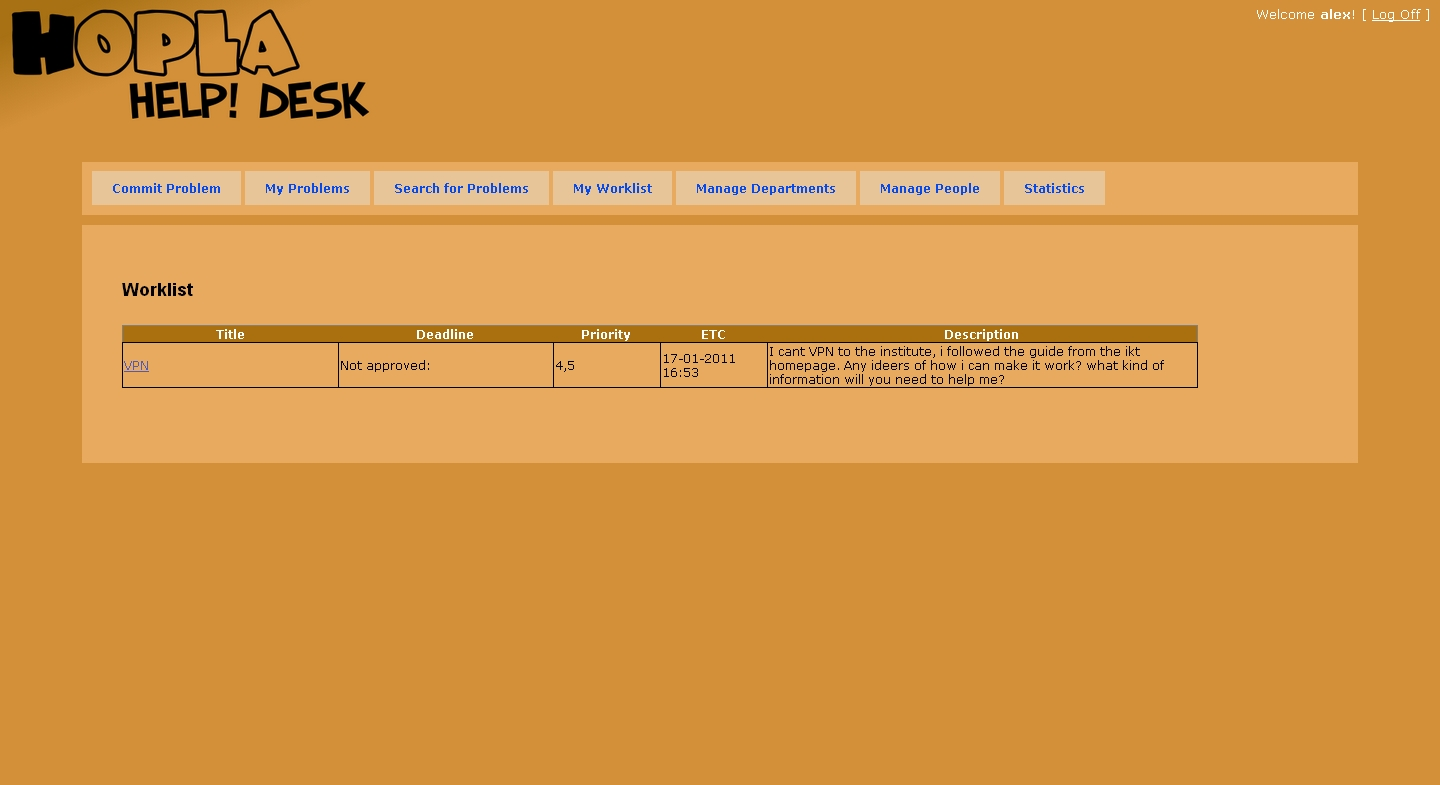
\includegraphics[width=1.00\textwidth, clip=true, trim=4cm 11.5cm 8cm 8cm]{input/alex_after.png}
	\label{fig:alex_after}
\end{figure}

\begin{figure}[H]
	\centering
		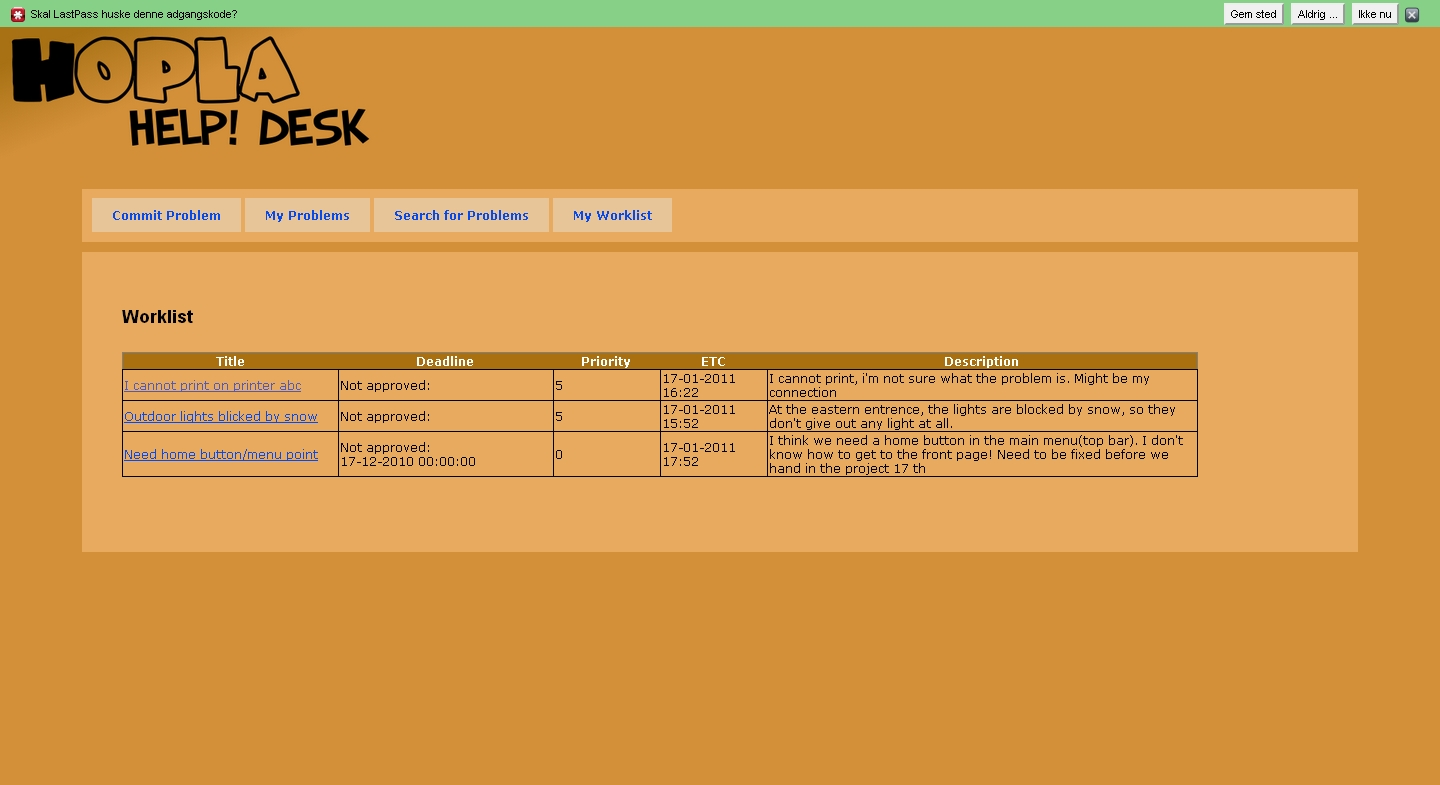
\includegraphics[width=1.00\textwidth, clip=true, trim=4cm 10.5cm 8cm 9cm]{input/magnus_after.png}
	\label{fig:magnus_after}
\end{figure}
\end{frame}

\subsubsection*{Balance Workload}
\begin{frame}{Balance Workload}
\only<1>{
\begin{itemize}
	\item Iterating $n-1$ times
	\begin{itemize}
		\item $n$ is the number employees in department
	\end{itemize}
	\item Balance between maximum and minimum workload
\end{itemize}
}
\only<2>{
\begin{figure}
	\centering
		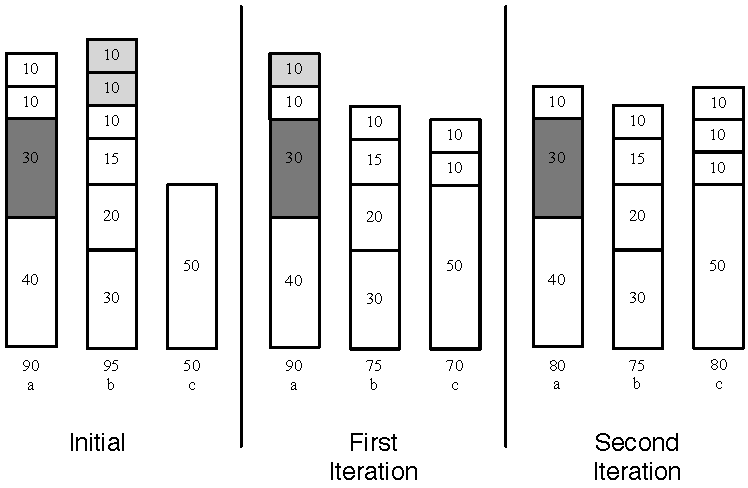
\includegraphics[scale=0.5]{input/balanceWorkloadDiagram.pdf}
	\caption{Found on page 80}
	\label{fig:balanceWorkloadDiagram}
\end{figure}
}
\end{frame}

\begin{frame}{Balance Workload -- Improvements}

\begin{itemize}
	\item Consider priority

	\begin{enumerate}
		\item<2-> Put all reassignable, unsolved problems into a list
		\item<3-> Sort the list
		\item<4-> Assign must important problem to least occupied person
		\item<5-> Repeat step 3 until all problems are assigned
	\end{enumerate}

\end{itemize}

\end{frame}
\subsection{Statistics}
\begin{frame}{Statistics}

\begin{itemize}
\item <1-> Current implementation
	\begin{itemize}
	\item<2-> Primitive
	\item<3-> Based on unsound data
	\end{itemize}
\end{itemize}

\begin{figure}[htbp]
	\begin{center}
	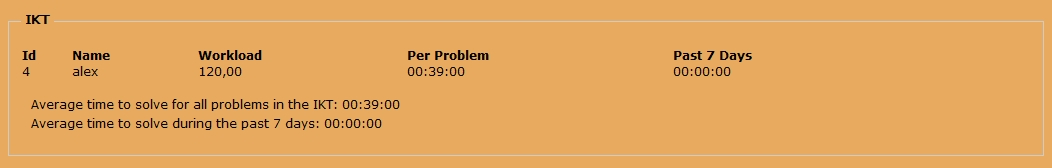
\includegraphics[width=280pt]{input/statistics.jpg}
	%\caption{default}
	%\label{default}
	\end{center}
\end{figure}

\end{frame}

\begin{frame}{Statistics}

\begin{itemize}
\item<1-> Potential improvements
	\begin{itemize}
	\item<2-> Better data:
		\begin{itemize}
		\item<3-> Time solving problems
		\item<4-> Type of problem
		\end{itemize}
	\item<5-> More factors:
		\begin{itemize}
		\item<6-> ``difficulty'' of the submitter
		\item<7-> Working hours of staff
		\end{itemize}
	\item<8-> Better UI
		\begin{itemize}
		\item<9-> Graphical presentation of data
		\item<10-> Show the average time on tags
		\end{itemize}
	\end{itemize}
\end{itemize}

\end{frame}
\section{Test}
\begin{frame}

\end{frame}
\section{Tests}
\begin{frame}{}
\begin{center}
\huge
Tests
\end{center}
\end{frame}
\subsection{Test Methods}
\begin{frame}{Test Methods}
	\begin{itemize}
		\item Black box testing
		\item White box testing
		\item Unit testing
		\begin{itemize}
				\item Visual Studios -- Team Test
		\end{itemize}
		\item Regression testing
	\end{itemize}
\end{frame}

\begin{frame}{Test Methods}
	\begin{itemize}
		\item Balance Workload
			\begin{enumerate}
				\item Unit testing
				\item White box testing
				\item Dependency Injection
				\item Regression Testing
			\end{enumerate}
		\item Problem Search
		\begin{enumerate}
				\item Unit testing
				\item White box testing
			\item Code coverage
			\begin{itemize}
			\item Figure 15.2
			\end{itemize}
			\item Regression testing
		\end{enumerate}
	\end{itemize}
\end{frame}
\chapter{Conclusion}
\label{chap:conclusion}
We initiated this project with a partly comprehensive project proposal which meant that we could start the analyzation-phase immediately. This went hand-in-hand with the \ooad{} method which the study regulation required that we used. The \ooad{} method resulted in a comprehensive analysis and design phase, which we documented immediately afterwards. We afterwards chose to useuse the MVC design pattern, which -- due to the programming language of choice, C# the ASP.NET MVC 2 framework, which took a relatively big amount of time to learn. During this learning phase, we realized that we had to redo and change alot of the decisions we made during the design phase, as well as reinterpret some parts from the analysis, in order to use the ASP.NET MVC 2 framework for our implementation. Due to the limited amount of time we had left, we were forced to make these decisions, which not always led to a better and more intuitive application. This led to a rather large improvements chapter (chapter \ref{chap:future_work}). We did not document our developed application until we decided that we were done developing, whereafter the remaining time were spent documenting our application, as well as decisions which were made during the development part.


%The goal of this project is to use the knowledge gained from the two courses SAD and OOP. The approach to achieve this is to make a application based upon the materials learned from the two courses. This resulted in a throughly analysis and design instead of spending time of learning how the ASP.NET MVC2 framework works. Which meant that a lot of the time we initially spent on the design were completely wasted as we realized that it could not be implemented properly using the framework. Therefore we started very late on the implementation and did not use the required time to throughly make a full system test and correct all bugs. This could be avoided by achieving knowledge of the framework prior to the design phase. 




%In general we used a lot of new technologies which we had a very sparse knowledge of and this resulted in parts of the system were we afterwards can see that this could have been done more comprehensible and efficient. The whole learning process of this project has been trial and error. We tried applying new technologies and sometimes it went well or if not we learned something from it. 



\end{document}